% !TEX root =  ../main_manuscript.tex

\subsection{Personalized Decisions for Biopsy}
\label{subsec:pers_decision_making}
Let us assume that a decision of conducting a biopsy is to be made for a new patient $j$ shown in Figure~\ref{fig:obsDataPlot_2340}, at his current follow-up visit time $s$. Let $t\leq s$ be the time of his latest negative biopsy. Let $\mathcal{Y}_{dj}(s)$ and $\mathcal{Y}_{pj}(s)$ denote his observed DRE and PSA measurements up to the current visit, respectively. From the observed measurements we want to extract the underlying measurement error free trend of $\log_2 (\mbox{PSA} + 1)$ values and velocity, and the log odds of obtaining $\mbox{DRE} > \mbox{T1c}$. We intend to combine them to inform us when the cancer progression is to be expected (see~Figure~\ref{fig:dynRiskPlot_2340}), and to further guide the decision making on whether to conduct a biopsy at the current follow-up visit. The combined information is given by the following posterior predictive distribution $g(T^*_j)$ of his time of cancer progression $T^*_j > t$ (see~Appendix~A.4 for details):
\begin{equation}
\label{eq:post_pred_dist}
g(T^*_j) = p\big\{T^*_j \mid T^*_j > t, \mathcal{Y}_{dj}(s), \mathcal{Y}_{pj}(s), \mathcal{D}_n\big\}.
\end{equation}
The distribution $g(T^*_j)$ is not only patient-specific, but also updates as extra information is recorded at future follow-up visits.

\begin{figure}[!htb]
\captionsetup{justification=justified}
\centerline{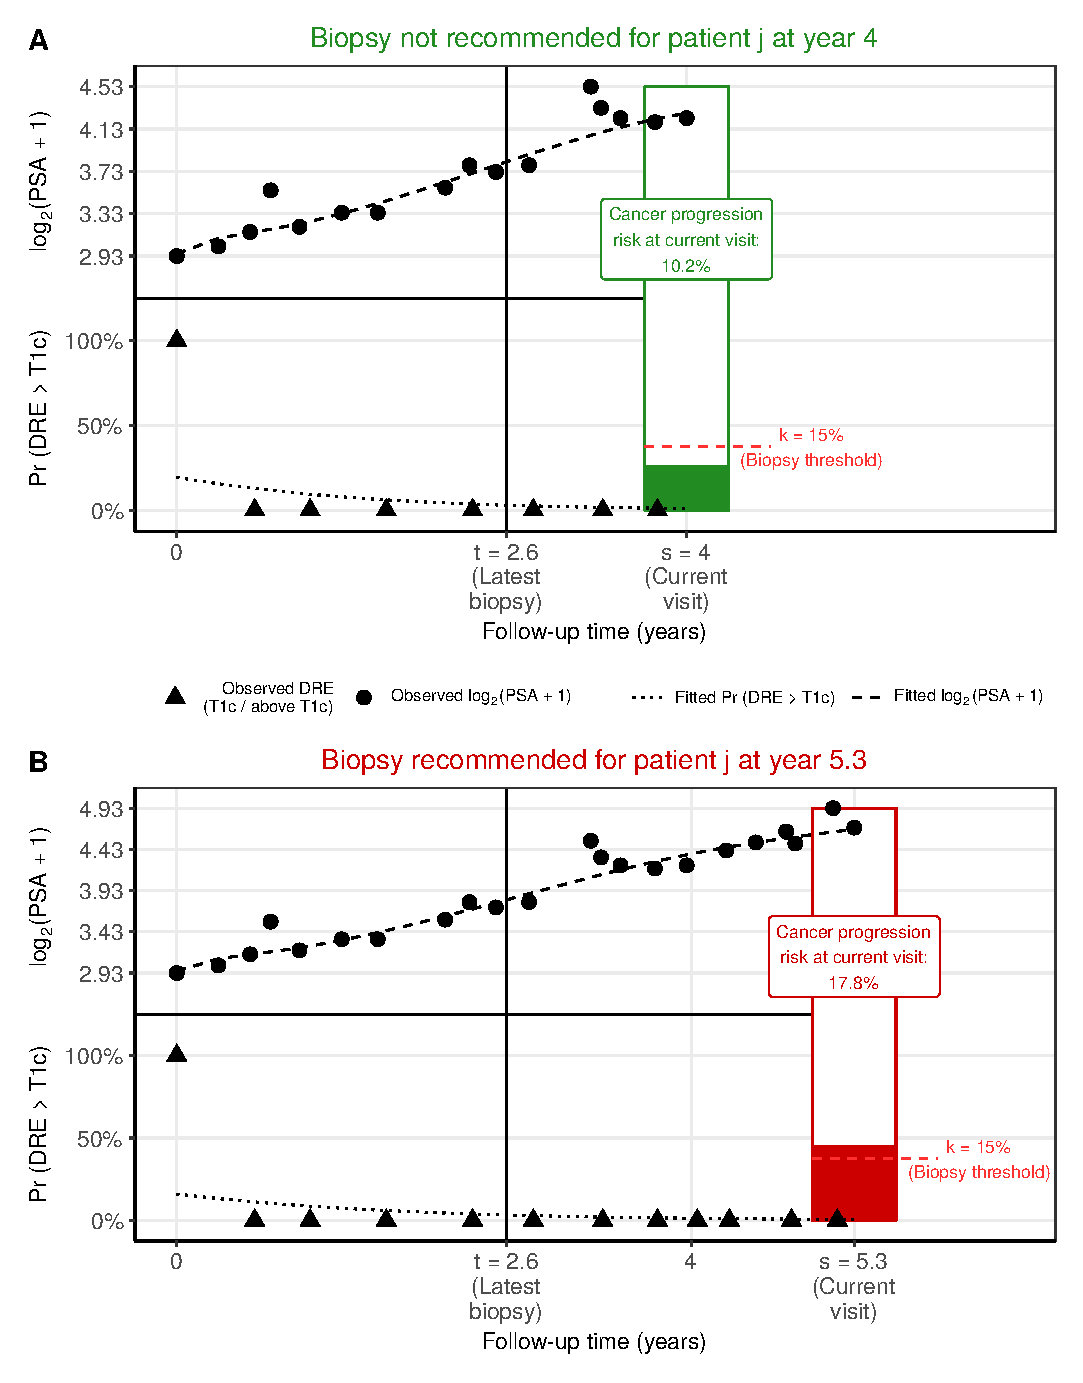
\includegraphics[width=\columnwidth]{images/dynRiskPlot_2340.eps}}
\caption{\textbf{Illustration of personalized decision of biopsy} for patient $j$ at two different follow-up visits. Biopsy is recommended if the personalized cumulative risk of cancer progression estimated from the joint model fitted to the observed data of the patient, is higher than the example risk threshold for biopsy ($\kappa=$ 10\%). \textbf{Panel~A:} biopsy is not recommended for the patient $j$ at the follow-up visit time $s=4$ years, because his estimated personalized cumulative risk of cancer progression (7.8\%) is less than the threshold. \textbf{Panel~B:} biopsy is recommended for the patient $j$ at the follow-up visit time $s=5.3$ years, because his estimated personalized cumulative risk of cancer progression (13.5\%) is more than the threshold.}
\label{fig:dynRiskPlot_2340}
\end{figure}

A key ingredient in the decision of conducting a biopsy for patient $j$ at the current follow-up visit time $s$ is the personalized cumulative risk of observing a cancer progression at time $s$ (illustrated in Figure~\ref{fig:dynRiskPlot_2340}). This risk can be derived from the posterior predictive distribution $g(T^*_j)$ \cite{rizopoulos2011dynamic}, and is given by:
\begin{equation}
\label{eq:dynamic_risk_prob}
R_j(s \mid t) = \mbox{Pr}\big\{T^*_j \leq s \mid T^*_j > t, \mathcal{Y}_{dj}(s), \mathcal{Y}_{pj}(s), \mathcal{D}_n\big\}, \quad s \geq t.
\end{equation}
A simple and straightforward approach to decide upon conducting a biopsy for patient $j$ at the current follow-up visit would be to do so if his personalized cumulative risk of cancer progression at the visit is higher than a certain threshold $0 \leq \kappa \leq 1$. For example, as shown in Panel~B of Figure~\ref{fig:dynRiskPlot_2340}, biopsy at a visit may be scheduled if the personalized cumulative risk is higher than 10\% (example risk threshold). This decision making process is iterated over the follow-up period, incorporating on each subsequent visit the newly observed data, until a positive biopsy is observed. Subsequently, an entire personalized schedule of biopsies for each patient can be obtained.

%Although, the number of unnecessary biopsies a risk threshold may eventually lead to is related to its accuracy of classification between patients whose cancers have progressed and patients without cancer progression. The classification accuracy of a risk threshold also varies over the follow-up period.

The choice of the risk threshold dictates the schedule of biopsies and has to be made on each subsequent follow-up visit of a patient. In this regard, a straightforward approach is choosing a fixed risk threshold, such as 5\% or 10\% risk, at all follow-up visits. Fixed risk thresholds may be chosen by patients and/or doctors according to how they weigh the relative harms of doing an unnecessary biopsy versus a missed cancer progression (e.g., 10\% threshold means a 1:9 ratio) if the biopsy is not conducted \cite{vickers2006decision}. An alternative approach is that at each follow-up visit a unique threshold is chosen on the basis of its classification accuracy. More specifically, given the time of latest biopsy $t$ of patient $j$, and his current visit time $s$\, we find a visit-specific biopsy threshold $\kappa$, which gives the highest cancer progression detection rate (true positive rate, or TPR) for the period $(t, s]$. However, we also intend to balance for unnecessary biopsies (high false positive rate), or a low number of correct detections (high false negative rate) when the false positive rate is minimized. An approach to mitigating these issues is to maximize the TPR and positive predictive value (PPV) simultaneously. To this end, we utilize the $\mbox{F}_1$ score, which is a composite of both TPR and PPV (estimated as in Rizopoulos~et~al., 2017 \cite{landmarking2017}), and is defined as: 
\begin{equation}
\label{eq:F1_TPR_PPV}
\begin{split}
\mbox{F}_1(t,  s, \kappa) &= 2\frac{\mbox{TPR}(t,  s, \kappa)\ \mbox{PPV}(t,  s, \kappa)}{\mbox{TPR}(t,  s, \kappa) + \mbox{PPV}(t,  s, \kappa)},\\
\mbox{TPR}(t,  s, \kappa) &= \mbox{Pr}\big\{R_j(s \mid t) > \kappa \mid t < T^*_j \leq s\big\},\\
\mbox{PPV}(t,  s, \kappa) &= \mbox{Pr}\big\{t < T^*_j \leq s \mid R_j(s \mid t) > \kappa \big\},
\end{split}
\end{equation}
\textcolor{blue}{where, $\mbox{TPR}(t,  s, \kappa)$ and $\mbox{PPV}(t,  s, \kappa)$ are the time dependent true positive rate and positive predictive value, respectively. These values are unique for each combination of the time period $(t, s]$ and the risk threshold $\kappa$ that is used to discriminate between the patients whose cancer progresses in this time period versus the patients whose cancer does not progress. The same holds true for the resulting $\mbox{F}_1$ score denoted by $\mbox{F}_1(t,  s, \kappa)$. The $\mbox{F}_1$ score ranges between 0 and 1, where a value equal to 1 indicates perfect TPR and PPV. Thus the highest $\mbox{F}_1$ score is desired in each time period $(t, s]$. This can be achieved by choosing a risk threshold $\kappa$ which maximizes $\mbox{F}_1(t, s, \kappa)$. That is, during a patient's visit at time $s$, given that his latest biopsy was at time $t$, the visit-specific risk threshold to decide a biopsy is given by ${\kappa=\argmax_{\kappa} \mbox{F}_1(t, s, \kappa)}$. The criteria on which we evaluate the personalized schedules based on fixed and visit-specific risk thresholds is the total number of biopsies scheduled, and the delay in detection of cancer progression (details in \hyperref[sec:results]{Results}).}